\documentclass{article}
\usepackage{authblk}
\usepackage{acro}
\usepackage{amsmath}
\usepackage{amsfonts}
\usepackage{caption}
\usepackage{ccaption}
\usepackage[margin=20truemm]{geometry}
\usepackage[dvipdfmx]{graphicx}
\usepackage{hyperref}
\usepackage{url}

\title{
  A graph-based practice of evaluating collective identities of cell clusters
}
\author[1,2]{Yuji Okano}
\author[2]{Yoshitaka Kase}
\author[2]{Hideyuki Okano}
\affil[1]{
  Department of Extended Intelligence for Medicine, 
  The Ishii-Ishibashi Laboratory, 
  Keio University School of Medicine
}
\affil[2]{
  Division of CNS Regeneration and Drug Discovery,
  International Center for Brain Science, 
  Fujita Health University
}
\date{\today}

\DeclareAcronym{scRNA-seq}{short = scRNA-seq, long  = single-cell RNA-sequencing}
\DeclareAcronym{GRN}{short = GRN, long  = gene regulatory network}
\DeclareAcronym{JIM}{short = JIM, long  = Jaccard index matrix}
\DeclareAcronym{DEA}{short = DEA, long  = differential expression analysis}
\DeclareAcronym{DEG}{short = DEG, long  = differentially expressed gene}
\DeclareAcronym{PC}{short = PC, long  = Peter and Clark}
\DeclareAcronym{RPM}{short = RPM, long  = reads per million}
\DeclareAcronym{HVG}{short = HVG, long  = highly variable gene}
\DeclareAcronym{PCA}{short = PCA, long  = principal component analysis}
\DeclareAcronym{TSVD}{short = TSVD, long  = truncated singular value decomposition}
\DeclareAcronym{UMAP}{short = UMAP, long  = Uniform Manifold Approximation and Projection}
\DeclareAcronym{ML}{short = ML, long  = machine learning}
\DeclareAcronym{GBDT}{short = GBDT, long  = gradient boosting decision tree}
\DeclareAcronym{GO}{short = GO, long  = gene ontology}
\DeclareAcronym{QC}{short = QC, long  = quality control}
\DeclareAcronym{MMHC}{short = MMHC, long  = max-min hill-climbing}

\DeclareCaptionLabelFormat{mainfigs}{\textbf{Figure #2}}
\captionsetup[figure]{labelformat=mainfigs}

\urlstyle{same}

\begin{document}

\maketitle

\section*{Abstract}
Random sentences

\section*{Introduction}
It has been more than 10 years since the birth of \ac{scRNA-seq}\cite{tang2009mrna}, and the technology now 
is recognized as a prominent game changer of the molecular biology of this decade. Likewise the pioneering technologies, DNA 
micro array and bulk RNA-seq, scRNA-seq can observe multidimensional gene expression profiles, while it also can 
provide such information in single-cell-level. Although this informative assay have contributed to reveal detailed 
biology of various cell types, the excessive resolution blurred the conceptual boundary between static cell types and 
transient cell status\cite{regev2017human}. Consequently, clusters, chunks of samples that shares similar geometrical properties in the 
data space overwrote the classical notion of cell types. As the cell clusters are dependent on sampling stochasticity 
of the dataset, and their biological properties might sway from the original doctrine of cell types\cite{okano2023set}. Hence, a theoretical 
backbone and a effective method to glue the theory and real data are essential to identify universal characters of specific 
samples from piles of extrinsic noises.

In our previous research, we proposed a \ac{GRN}-based representation of cell clusters 
while edges of GRNs explain statistical dependencies between two genes, and demonstrated that similarity of two 
clusters can be defined as a quasi-pseudo-metric function $d^*$\cite{okano2023set}. To discuss mathematical properties of the space of 
cell clusters, we defined novel terms, cell class and eigen-cascades, and step-by-step introduced their algebraic 
structures. Eigen-cascades refer to a set of marker genes and pairs of genes that are statistically dependent (i.e., 
isomorphic to the direct sum of the direct sums of the vertex set and the edge set of a GRN). A cell class refers to 
a cell cluster characterized with the corresponding eigen-cascades. Note that the nuances of cell clusters and cell 
classes are slightly different even though we might use those terms interchangeably in this article (See Appendix 
for more descriptions). When two cell classes $^\forall[x], [y]$ are represented by the GRNs regarding a set of genes $G$, and 
the two GRNs (eigen-cascades) respectively denoted as $C_{[x]}(G)$ and $C_{[y]}(G)$, a bivariate function $d^*$ that maps a 
pair of cell classes to real numbers are defined as follows\cite{okano2023set}:
\begin{equation}\label{d_asterisk}
  d^*([x], [y]) := 1 - \frac{|C_{[x]}(G)\cap C_{[y]}(G)|}{|C_{[x]}(G)|}.
\end{equation}
Eq. \eqref{d_asterisk} is derived from the Hamming distance function (a metric function that measures the difference of two 
character strings) and modified to embrace the tendency of the \ac{PC} algorithm, one of the most 
simple bayesian network algorithms\cite{okano2023set,bookstein2002generalized, spirtes2000causation}. With those concepts, we also proposed frameworks to compare the 
similarities of given two cell clusters. Our scheme comprises two fundamental steps: formation of GRNs and 
evaluation of their similarity (\figurename{ 1A}). As the concept of cell classes are independent from the choice of data 
analysis methods, this framowork itself can be applied into various cases regardless of any feature engineering (such 
as the data preprocessing) and clustering methods.

The framework can be applied into the annotation of scRNA-seq data when a referential dataset is available 
(\figurename{ 1B}). As the annotation is the act of tagging clusters with descriptions in natural languages, the biological 
features of annotated clusters often treated as general and preserved properties of the cell types which the clusters 
are named after. Accordingly, it is better to have a large enough referential dataset which seem to reflect canonical 
states of specific cell types which are shared with the query dataset. Using GRN-based characterization, cell classes 
are annotated with the name of the most similar cell class, however, comparisons of cellular identities can be 
bidirectional due to asymmetry of $d^*$. We named the similarity of cell classes from the perspectives of the query 
data as estimation, and the one from the point of view of the referential data as labeling. Those GRN-based 
annotations can be visualized with planet plots, where the subjective cell class (here we denote it $[x]$) is located in 
the center and the radii of the circles reflect $d^*([x],\cdot)$ values for all cell classes placed on the circumferences.

The performance of those frameworks build around GRNs have its bottleneck in the step to create GRNs, and 
the process can be broken down into the configuration of the vertex sets and the choice of the network algorithm 
(\figurename{ 1C}). As well as the methods of the feature engineering and the clustering, each step of the GRN formation 
also has a variety of options. In the last paper, we introduced a combined method of manual curation referring 
review articles and a \ac{ML}-based feature selection using a \ac{GBDT} 
model with the L1 and the L2 regularizations\cite{okano2023set}. For the manual supervision, \ac{GO} terms can be 
another information source. Nevertheless, a priori identification of the sample components are essential to create 
meaningful GRNs by injecting the domain-specific information. The \ac{DEG}-based 
method can be a more heuristic and a less interactive option because the \ac{DEA} 
semi-automatically scoops DEGs. Regarding the network algorithms, we mentioned that there are several possible 
options as well. In our previous paper, we implemented our codes using the numerical (i.e., correlation-based) PC 
algorithms provided in Pgmpy\cite{pgmpy}, a python package for probablistic graphical models. Another variation of the PC 
algorithm based on the chi-square test suitable for categorical data is also a realistic option if when the expression 
values can be binalized in some ways. We also mentioned that the \ac{MMHC} algorithm, which 
combines constraint-based and scoring-based methods\cite{tsamardinos2006max}, is one of promissing alternatives of the PC algorithm.

\begin{figure}[htb]
  \centering
  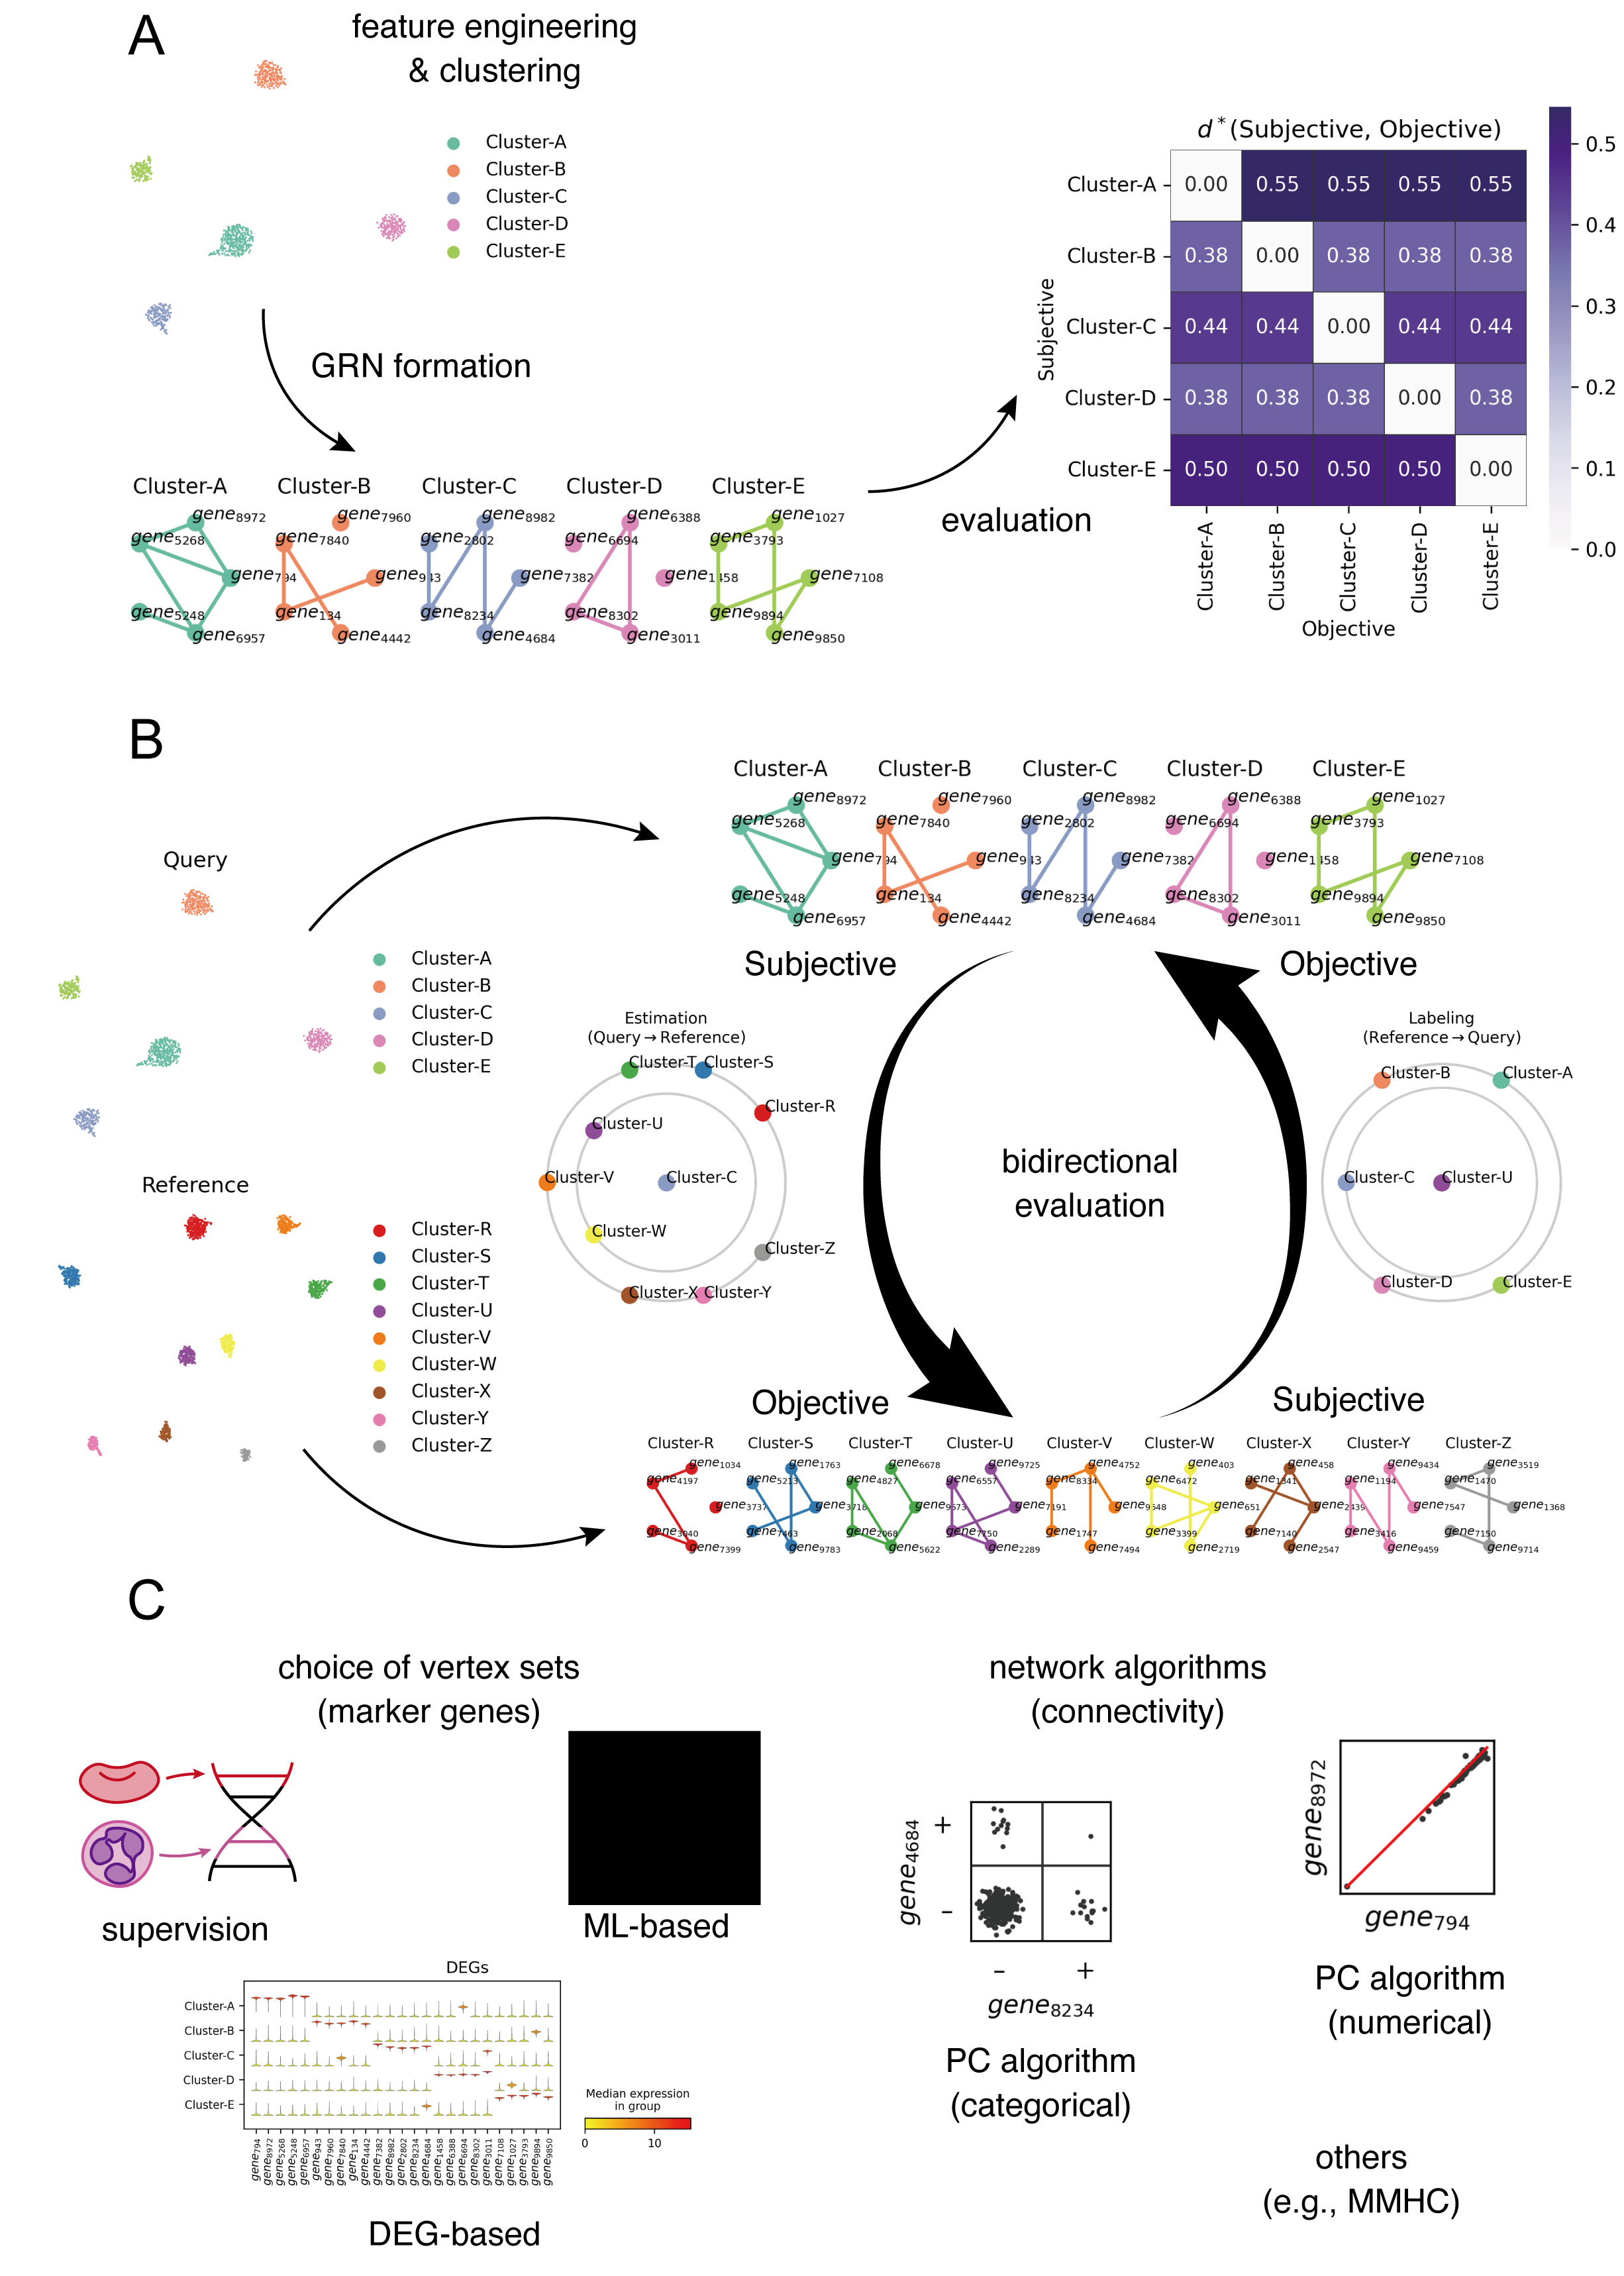
\includegraphics[scale=0.7]{./figs/exported/figure_1.png}
  \caption{The framework of the GRN-based characterization and annotation of cell classes}
  \legend{
    \textbf{A}: The foundation of the GRN-based characterization of cell classes. 
    After clustering in designed data space by arbitrary methods, cell classes (the clusters) can be represented by 
    GRNs of corresponding genes of choice. The similarity of two GRNs of the same vertex 
    (marker gene) are evaluated with the assymetrical function $d^*$, where the return values 
    reflects the similarity from the viewpoint of the subjective clusters. \textbf{B}: 
    Schematic of the GRN-based scRNA-seq data annotation. Expecting the referential data to reflect canonical 
    states of target sample domains, the evaluation of the similarity among cell classes can be performed bidirectionally.
    \textbf{C}: Methodological variations of the selection of vertex sets (marker genes) and the algorithms to compute 
    the network structures of GRNs.
  }
  \label{framework}
\end{figure}

So far, we have highlighted the versatility of our framework by providing examples that showcase its applicability 
across various data analysis methods. Our intention was to allow researchers to reflect their expertise in specific 
sample domains or preferences to the process of describing the samples with words of biology. This customization 
ensures that the metrics for cellular identities are crafted to align with the specific research scopes, providing both 
necessary and sufficient resolutions. However, this design choice has the drawback of making our algorithm less 
user-friendly, as it requires a significant amount of effort in annotation, even when it might not be the primary 
focus of their projects. To validate the legitimacy of our theory in as many cases as possible, it is essential to refine 
the practices related to GRN-based annotation, streamlining the overall workflow.

In this article, enumerating the three major topics where the former protocol has rooms for refinement, we 
provided more prectical solutions for each while leveraging the backbone theory of GRN-based comparisons of cluster-wise
cellular identities (i.e., cell classes).

\section*{Results}
\subsection*{Challenges of the framework of GRN-based methods}
In this reserch, we revisited the workflow of the GRN-based annotation

$\vdots$

To demonstrate those difficulties, we analyzed an open source scRNA-seq data of peripheral blood mononuclear 
cells from 10X Genomics (for short, we named the dataset PMBC3k in this research).

\subsubsection*{1. Difficulty of effective gene selection}
In our previous study, we proposed a method to combine supervised curation reffering a review paper and a 

$\vdots$

The standard workflow consists the \ac{QC} of the data, normalization such as \ac{RPM} transformation and logarithmic transformation, \ac{HVG} extraction, demensionality reduction such as \ac{PCA}, 
\ac{TSVD}, \ac{UMAP}\cite{umap}, etc., clustering, \ac{DEA}, annotation, and other downstream analysis (\figurename{ S1}).

Considering the fact that 
our method's primary application is the annotation of scRNA-seq data, 
we need an alternative method to find marker genes to reduce computational costs and 
streamline the overall time required to initiate main analyses.

\subsubsection*{2. Statistical issue: independence v.s. uncorrelation}
The statistical independence of two events $A$ and $B$ is defined as a situation where the following equation holds:
\begin{equation}\label{independence}
  P(A\cap B)=P(A)P(B),
\end{equation}
where $P(\cdot)$ is the probability of an event. On the other hand, the correlation coefficient $Corr(X, Y)$ of stochastic variables 
$X$ and $Y$ is defined as follows:
\begin{equation}\label{corr}
  Corr(X, Y):=\frac{Cov(X, Y)}{\sqrt{Var[X]Var[Y]}}=\frac{E[(X-E[X])(Y-E[Y])]}{\sqrt{Var[X]Var[Y]}},\quad \text{if}\; Var[X]Var[Y] > 0,
\end{equation}
where $E[\cdot]$ is the expected value, $Var[\cdot]$ is the variance, and $Cov(\cdot, \cdot)$ is the covariance. Independent variables 
exhibit a correlation coefficient of zero, the converse is false (e.g., when $X\sim U(-1, 1)$, where $U(-1, 1)$ refers to the uniform 
distribution over the interval from -1 to 1, $Corr(X, X^2)=0$ although $X$ and $X^2$ are dependent). Therefore, strictly 
speaking, it is not appropriate to substitute the chi-square test or the exact test with the t test of correlation.

However, we introduced a correlation-based algorithm to get GRNs compromising rigor in order to adjust to 
continuous gene expression values. To address this issue, we need to implement an effective method to binarize the 
gene expression values so that the new algorithm would rely on the statistical tests of independence. This update 
would make our algorithm align better to the original concept of our theory.

\subsubsection*{3. Irresponsibility to gene expression values}
To demonstrate this difficulty, we analyzed an open source scRNA-seq data of peripheral blood mononuclear 
cells from 10X Genomics (for short, we named the dataset PMBC3k in this research).

\begin{figure}[htb]
  \centering
  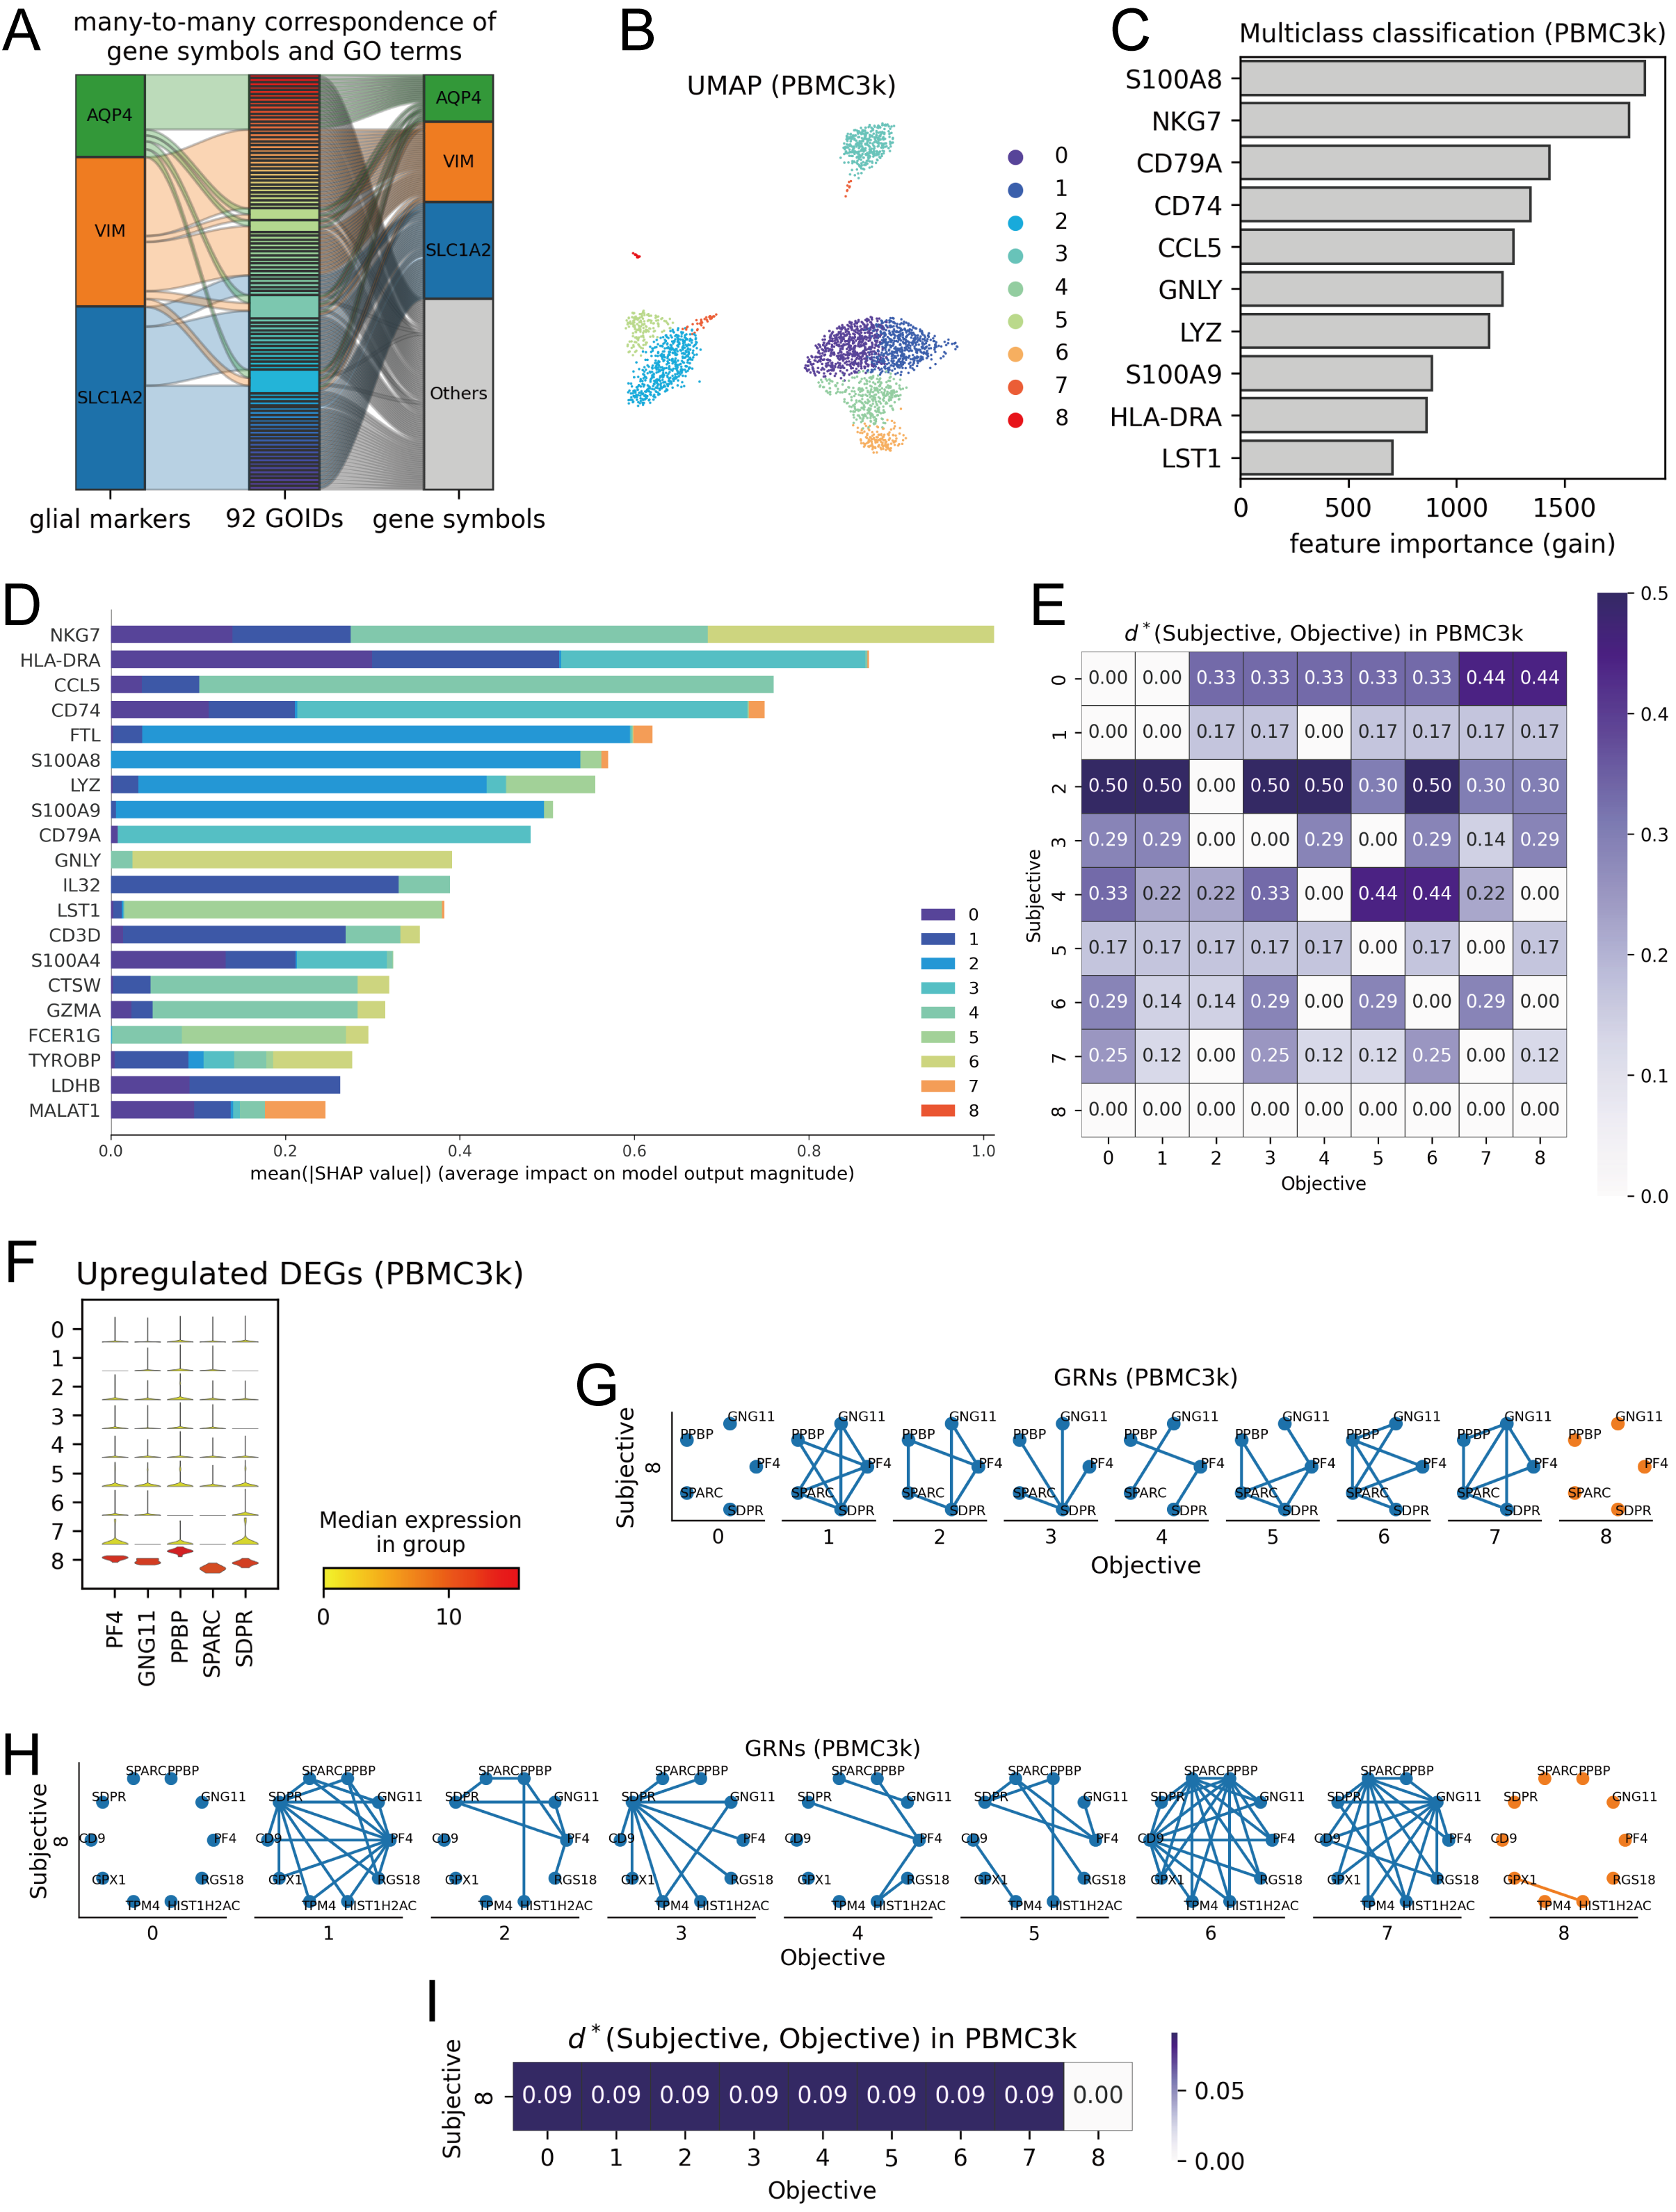
\includegraphics[scale=0.8]{./figs/exported/figure_2.png}
  \caption{Examples of the major issues on the GRN-based frameworks}
  \label{bc}
\end{figure}


\subsection*{Automated marker-gene suggestion}
Although we intended to require experimenters to curate marker genes to use
in GRNs, overly recurrsive trials to find 

\subsection*{Dropout-based binarization}
With a map $q: \Gamma\times X\rightarrow \mathbb{N}$ which returns a raw gene counts
of gene $^\forall g\in\Gamma$ for sample $^\forall x\in X$ where $\Gamma$ is the whole set of genes 
and $X$ is the whole set of samples, here we introduce the coverage function $Coverage_{[x]}: \Gamma\rightarrow\mathbb{Q}$ 
of cell class $[x]$ as follows:
\begin{equation}\label{coverage}
  Coverage_{[x]}(g):=\frac{
    |\{x\;|\;x\in[x]\;s.t.\;q(g,x)\neq 0\}|
  }{
    |[x]|
  }
\end{equation}
Note that $Coverage_{[x]}$ relies on $q$ only for identifying zeros in raw counts, therefore, 
any kind of values converted from raw counts by a transformation $\psi: \mathbb{N}\rightarrow\mathbb{R}$ 
such that $\psi^{-1}[\{0\}]=\{0\}$ can be used in lieu of $q(g, x)$. For instance, \ac{RPM} values 
and $\log_2(RPM+1)$ are accepted (see Appendix for more detailed explanations).

\subsection*{Weighted evaluation function}
\begin{equation}\label{HQPM}
  d^*([x], [y]) := 1 - \frac{|C_{[x]}(G)\cap C_{[y]}(G)|}{|C_{[x]}(G)|}
  =1 - \frac{
    |E_{[x]}(G)\cap E_{[y]}(G)|+|G|
  }{
    |E_{[x]}(G)|+|G|
  }
\end{equation}
\begin{equation}\label{WHQPM}
  Whqpm([x], [y]) := 1 - \frac{
    |E_{[x]}(G)\cap E_{[y]}(G)|+\sum_{g\in G}Coverage_{[x]}(g)
  }{
    |E_{[x]}(G)|+\sum_{g\in G}Coverage_{[x]}(g)
  }.
\end{equation}
Weighted Hamming quasi-pseudo-metric

\section*{Discussion}
I have no idea.

\section*{Methods}
\subsection*{GRNet Impletemtations}

\subsubsection*{GO term-assisted gene selection referring Jaccard Index}
\begin{equation}\label{jaccard}
  J(A, B) := \frac{A\cap B}{A\cup B}
\end{equation}
Jaccard Index of two sets $A, B$ is defined as Eq. \eqref{jaccard}. We expanded this 
definition to pairwise comparisons of multiple elements by forming a matrix 
where each element is the corresponding Jaccard Index, and we named the matrix \ac{JIM}. For example, the element in 
$i$-th row and $j$-th column (where $i, j, k\in\mathbb{N}$ and $i\leq k, j\leq k$), $JIM_{i,j}$, can be defined as
follows when a JIM of sets $X_1, X_2,\cdots, X_k$ are considered:
\begin{equation}\label{jim}
  JIM_{i, j} := J(X_i, X_j)
\end{equation}
Especially for seed markers, sets of subscribed GO terms (let $G_1, \cdots, G_k$)
and their JIM are calulated in order to set $min_{i,j}(J(G_i, G_j))$ as a threshold of 
biological correspondence.

$\vdots$

For detailed method of implementation, we calculated the JIM of the related GO terms of given seed markers. We used mygene.py\cite{mygene} to query the GO database, and Numpy\cite{numpy} to calculate JIM.

\subsubsection*{GRNs and the evaluation function}
Following our previous report\cite{okano2023set}, we computed GRNs by calculating
correlations of continuous gene expression values (e.g., $log_2(RPM+1)$) using pgmpy. In this study, we introduced

\subsection*{scRNA-seq data analysis}
\subsubsection*{Dataset List}
The scRNA-seq data we used in this research were publicly available as online
resources as follows:\\
M1C10X: \url{https://portal.brain-map.org/atlases-and-data/rnaseq/human-m1-10x}\\
hFB: \url{https://www.ncbi.nlm.nih.gov/geo/query/acc.cgi?acc=GSE165388}\\
PBMC3k: \url{https://support.10xgenomics.com/single-cell-gene-expression/datasets/1.1.0/pbmc3k}\\
aHSPC: \url{https://www.ncbi.nlm.nih.gov/geo/query/acc.cgi?acc=GSE137864}\\
BCA: \url{https://www.ncbi.nlm.nih.gov/geo/query/acc.cgi?acc=GSE149938}

\subsubsection*{Preprocessing, dimensionality reduction, and visualization}
We performed data preprocessing, dimensionality reduction, data visualization
of the scRNA-seq datasets using Python packages (including Scanpy\cite{scanpy}, Polars,
Pandas\cite{pandas}, Numpy, Matplotlib\cite{matplotlib}, Seaborn\cite{seaborn}) and Julia packages.

\subsubsection*{Clustering and DE analysis}
We performed leiden clustering, DE analysis using Scanpy.

\subsubsection*{Enrichment analysis}
We performed the enrichment analysis using gprofiler2\cite{gprofiler2}, and visualized the results with Matplotlib and Seaborn.

\subsection*{Other visualizations}
\subsubsection*{Alluvial plot of gene symbols and GO terms}
The glial markers were selected referring review articles, and the tagged GO terms were queried using mygene.py. 
Then, all gene symbols subscribed with each GO terms were queried again. The visualization was implemented 
with Matplotlib, Numpy, Pandas.

\section*{Resource availability}
\subsection*{Data availability}
Not applicable
\subsection*{Code availability}
GRNet and the analysis codes are available on GitHub (\url{https://github.com/yo-aka-gene/grnet}).
Online documentation for GRNet is also provived (\url{https://grnet.readthedocs.io}).


\section*{Author contributions}
YO designed the project, implemented the algorithms, excecuted the analyses, and wrote the manuscript. YK 
contributed as the senior author, and edited the manuscript. HO edited the manuscript, and supervised the project.

\section*{Acknowledgements}
We thank hogehoge for thorough support.


\section*{Abbreviations}
\printacronyms[heading=Abbreviations]

\bibliographystyle{ieeetr}
\bibliography{refs.bib}
\end{document}
